\section{Edge computing}
Edge computing is a subset of IOT research, which concerns itself with distributing the computational load across the devices at the edge of the of the network. Projections performed by forbes suggest that by 2025, more then 75 billion IOT devices will be connected to the Internet. As the devices at the edge become more computationally capable and more numerous, it becomes imperative to share the computational load not only across the cloud services, but across the devices themselves. Furthermore a large portion of these devices, such as home automation, do not require a connection to the cloud in the first place. Instead they require a connection to the edge IOT hub, or need the cloud service only to establish or broker communication with another IOT device.
\begin{figure}[h]
	\centering
	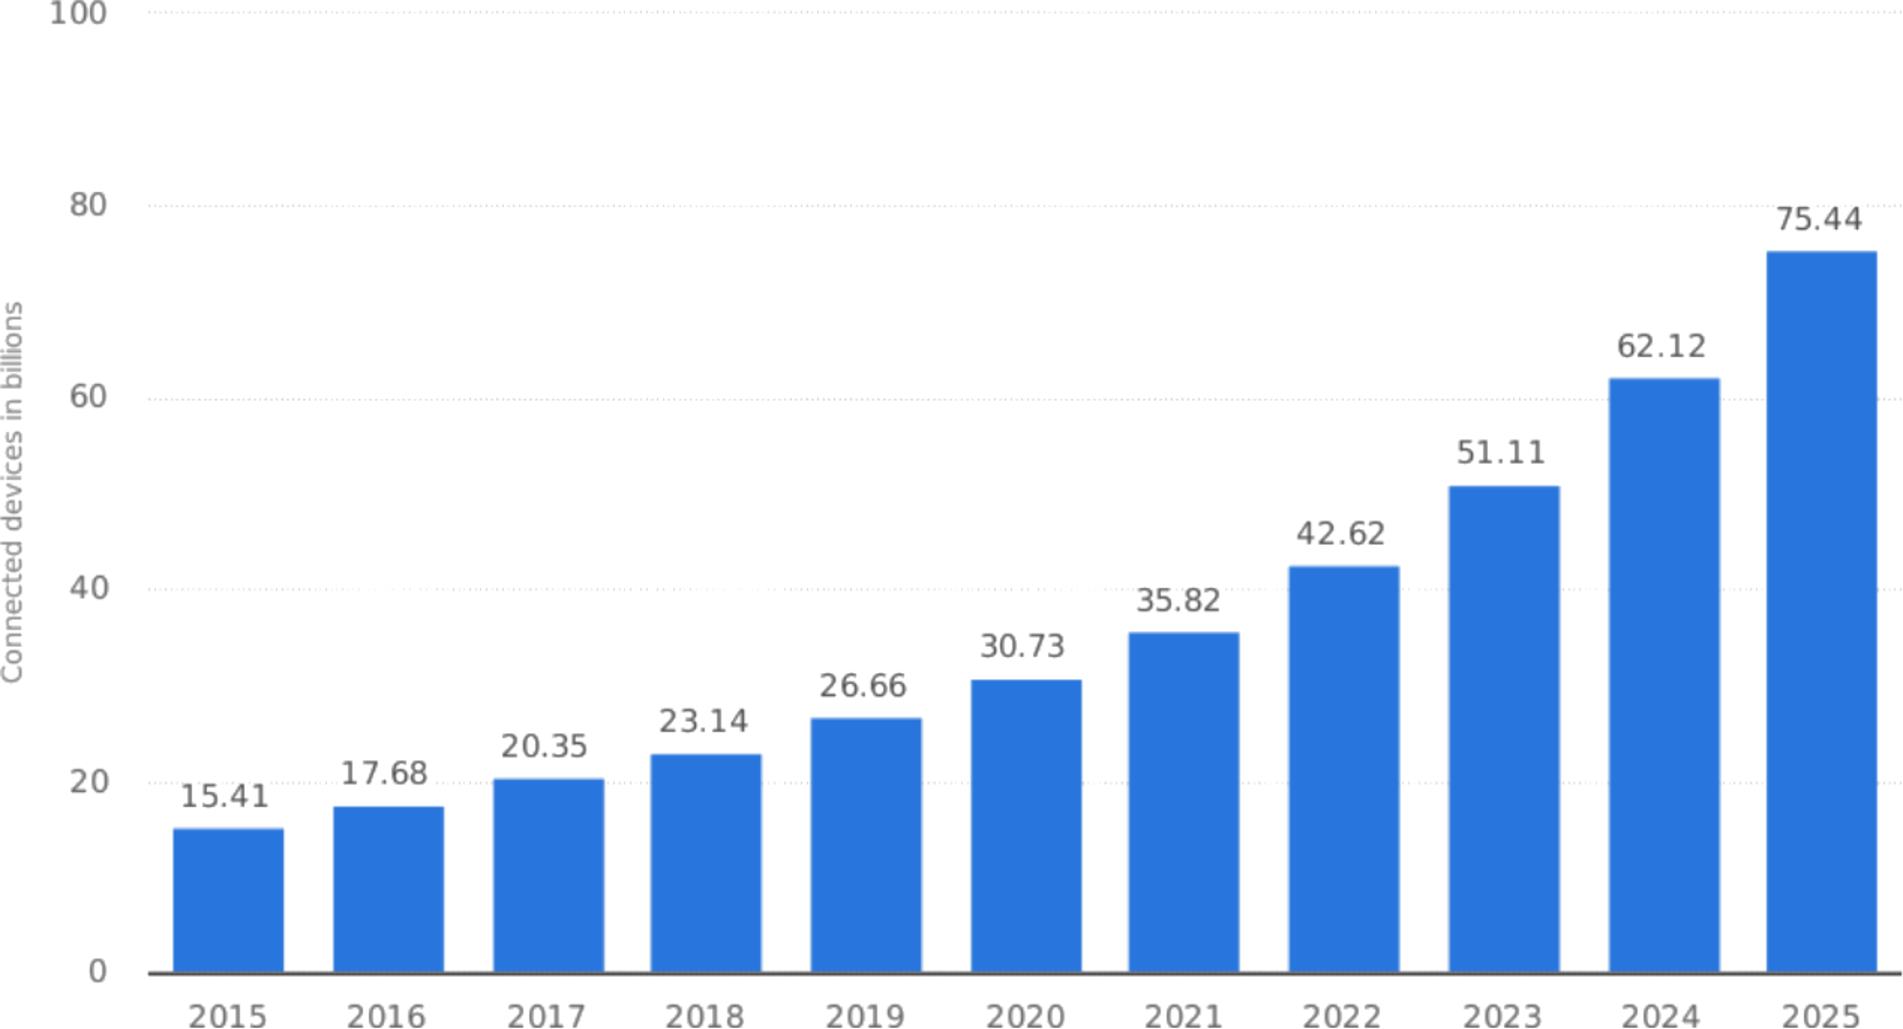
\includegraphics[width=0.8\linewidth]{img/iot_statistics.pdf}	
	\caption{Projected number of IOT devices worldwide}.
	\label{lit:fig:1}
\end{figure}

This change in communication strategy may seem inconsequential at first. However, upon deeper reflection in becomes clear that this is a major paradigm shift which brings IOT closer to the sensor network world it is often compared with. While the pioneering work in the IOT always assumed a one or two way communication between the IOT device and the cloud service, utilizing TCP/IP as an end-to-end protocol, it is becoming clear that this approach is unsustainable, and is often undesirable. This communication model has clear disadvantages in wasted communication, computation, and privacy. Furthermore the rigid computation communication model is not flexible enough to support devices which are beyond the edge of the TCP/IP network without an AD-HOC routing. 

The first attempt to address the bandwidth and latency issues arising with the widespread IOT adoption came in form of content delivery networks(CDNs). CDNs circumvent the generic cloud information delivery problems by placing transparent caches geographically spread across the application domain as shown in figure \ref{lit:fig:2}. When a user or an IOT device makes a request for on object, this request is forwarded to the nearest CDN node for processing. If the node contains the object in it's cache it is immediately forwarded to the requestee. Otherwise a request for the object is forwarded to the centralized cloud data store, and returned to the requesting device, as well as placed in the local cache. This approach has the advantage of moving the data closer to the end user, thus reducing latency, and taking advantage of the geographical locality. Another advantage of this method, is the added resiliency of the CDN architecture to single point failure. If a local cache node fails, it`s userbase, can be forwarded to another node, although encoring additional latency. Additionally if a centralized data store becomes unreachable, the local cache nodes can to some extent mask it's outage by forwarding the data available locally. This approach does have some drawbacks. While it makes it easier to enable faster transactions regarding data, it is not trivial to move application logic to the local cache nodes. Furthermore, CDN methodology, still relies on a central mediator for device communication, even if the devices are located in the same room. 

\begin{figure}[h]
	\centering
	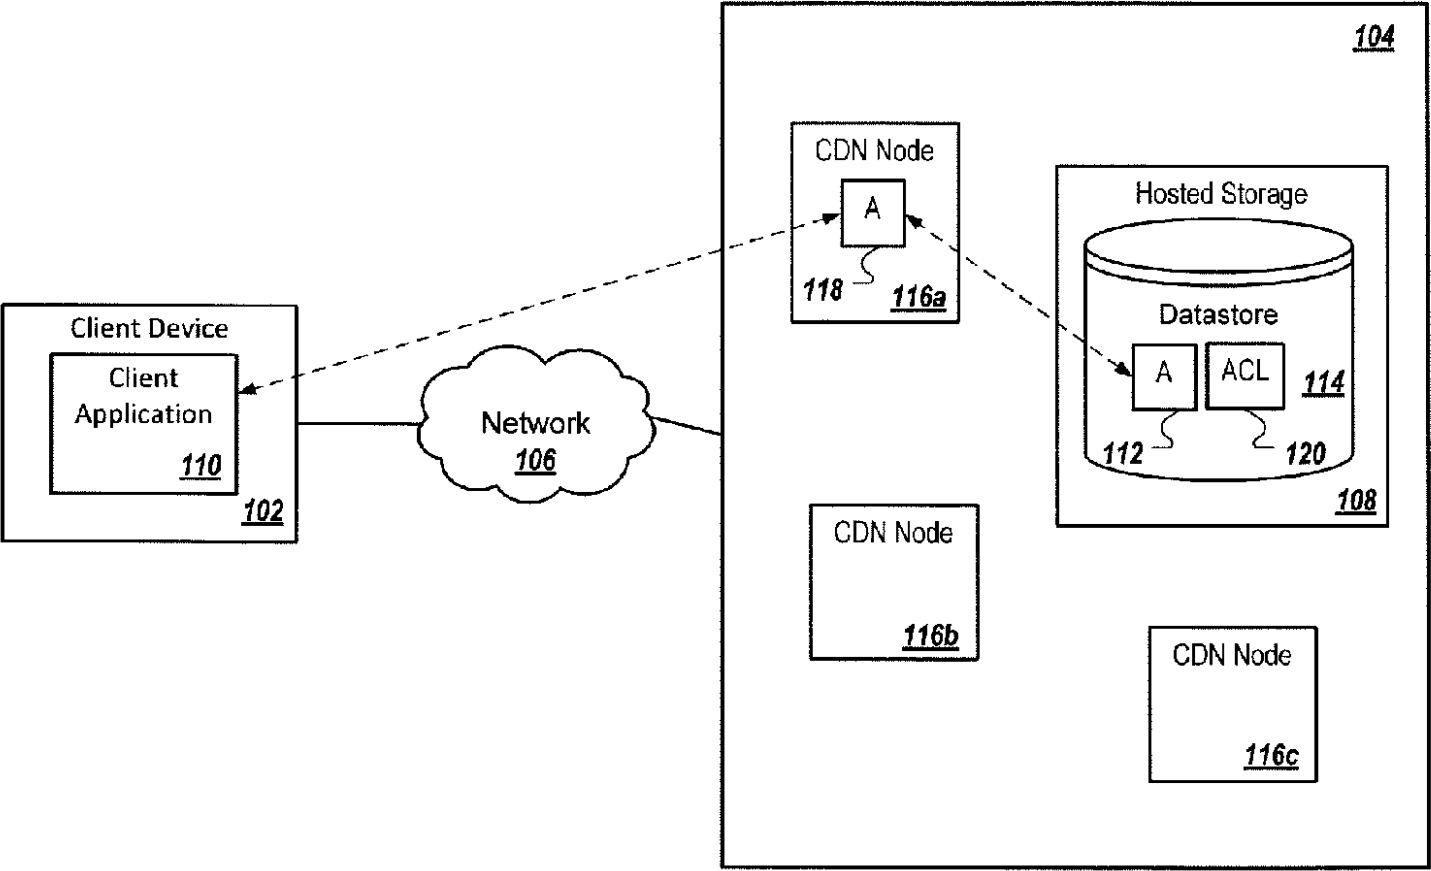
\includegraphics[width=0.6\linewidth]{img/cdn.png}	
	\caption{Content delivery network architecture. As described in the Google pattent.}.
	\label{lit:fig:2}
\end{figure}
